% Use draft for fast compile while editing; remove for final PDF
\documentclass[sigplan,10pt,nonacm]{acmart}

\AtBeginDocument{%
\providecommand\BibTeX{{Bib\TeX}}}

\usepackage{tikz}
\usepackage{graphicx}
\usetikzlibrary{arrows.meta,positioning,shapes.geometric}

\title{Recovering TASO Substitutions Under Bounded Rewrite Closure}

\author{Pietro Marsella}
\email{marsella@stanford.edu}

\author{Bodo Wirth}
\email{bodow@stanford.edu}

\renewcommand{\shortauthors}{Marsella and Wirth}

% TODO: be consistent: always call them substitutions, not rewrite rules.

\begin{document}

\begin{abstract}
Machine learning compilers have emerged in recent years as a major tool for automatically optimizing the performance of deep learning models. A major component of this optimization pipeline is \textbf{algebraic rewriting}, where a compiler repeatedly applies algebraic graph substitutions to transform a model into a semantically equivalent but more efficient form.

In several modern compilers, these substitutions are hand-written. Recent works such as TASO, however, have shown that substitutions can instead be discovered automatically by enumerating candidate graph pairs and then formally verifying the potentially valid ones using a smaller set of base operator axioms. In this paper, we study the following question: are these substitutions, given a powerful enough rewrite system, derivable as explicit compositions of the base TASO axioms? If so, the compiler pipeline could be simplified significantly by removing the need for a separate substitution discovery stage and instead relying on an expressive axiom set.

To answer this question, we design a powerful rewrite system over a symbolic graph IR and use it together with bounded search to find explicit axiomatic derivations for the substitutions discovered by TASO. Evaluated on 444 substitutions extracted from the TASO implementation, our system recovers over $97\%$ of them, with most derivations requiring only a small number of axiom applications. These results suggest that given a powerful enough rewrite system, most substitutions discovered by TASO are derivable from the base axioms.

The implementation is available at \url{https://github.com/Marsella8/taso-sparse}.
\end{abstract}
\maketitle

% \section{Introduction}
% Machine learning compilers have become a central part of the deep learning software stack. Their role is not only to lower models to kernels, but also to transform computation graphs into equivalent forms that execute more efficiently on the target hardware. At this level, one of the most important optimization mechanisms is algebraic rewriting: replacing a subgraph with a semantically equivalent one that yields lower cost under some objective, such as runtime, memory traffic, or communication volume. As deep learning systems have grown larger, more heterogeneous, and more distributed, the quality of these graph-level transformations has become increasingly important.

% A traditional way to build such optimizers is to hand-design a collection of graph substitutions. This requires substantial manual effort, scales poorly as the operator set grows, and makes it difficult to understand how much of the optimizer's behavior is really grounded in a small trusted semantic core. TASO addressed part of this problem by showing that useful graph substitutions can be generated automatically from a base set of operator axioms, then formally verified before being used in optimization~\cite{jia2019taso}. For the optimization step, TASO keeps a working set of equivalent graphs, sorted in order of cost, and greedily applies substitutions to the lowest cost graph for a predefined number of steps.

% Subsequent work focused largely on how to search more effectively over the space induced by such substitutions. MetaFlow observed that restricting attention to immediately profitable rewrites can be too limiting, and introduced relaxed graph substitutions that allow performance-decreasing intermediate steps in order to reach better final graphs~\cite{jia2019relaxed}. TENSAT instead performs equality saturation to compactly represent the equivalent graphs at once and thereby alleviate the phase-ordering problems of sequential rewriting~\cite{yang2021equality,willsey2021egg}. Unity extended the same perspective to distributed training, representing both algebraic transformations and parallelization choices as substitutions over a unified parallel computation graph~\cite{unger2022unity}. The effectveiness of these systems suggests that having a general framework for gneerating and applying substitutions outperforms hand-designed ones.

% This paper studies a complementary question. Rather than asking how to discover substitutions, or how to search over them once they are known, we ask whether, for some sufficiently powerful rewrite system, the substitutions discovered by TASO are already implicit in the bounded rewrite closure of TASO's own base axioms. This question matters for both methodology and engineering. If most discovered substitutions are derivable, then they can be viewed as lemmas induced by a comparatively small trusted core, rather than as independent primitive facts. If they are not derivable, then the gap points to limitations in the rewrite framework used to explore them.

% To investigate this question, we implement a bidirectional rewrite system over a symbolic graph IR and use it to reconstruct TASO substitutions under bounded rewrite closure. Our investigation leads to a rewrite system that is able to handle several adversarial cases, including surjective variable matching, tensor aliasing, dead node elimination, and multi-output matching. Using this system, we recover over 95\% of the substitutions discovered by TASO. Beyond the headline number, the reconstruction process also provides a structural view of the substitution set itself: many substitutions emerge naturally as short derived lemmas, some require unexpectedly long derivations, and a small residual set appears to lie outside the closure induced by the current axiom basis.

\section{Introduction}

Machine learning compilers have become a central part of the deep learning software stack. One of the initial steps of compilation, generally done on a high-level graph IR, is algebraic rewriting: from a set of predetermined substitutions, the compiler matches a substitution to a model and applies it, which effectively means taking a subgraph and replacing it with a semantically equivalent one. This yields models that are semantically equivalent but better according to some cost such as runtime, memory traffic, or latency.

A traditional way to build such substitution sets is to manually design them. This requires substantial manual effort, scales poorly as the operator set grows, and increases the likelihood of bugs as each substitution written independently. TASO addressed part of this problem by showing that useful substitutions can instead be discovered automatically and then formally verified from a smaller set of base operator axioms, before being used in optimization~\cite{jia2019taso}. This naturally leads to a further question: once TASO has discovered such substitutions, how many of them are already obtainable by repeatedly composing the original axioms inside an explicit rewrite system?

This paper studies that question. Rather than using SMT-based validation to prove that candidate substitutions are correct, we ask whether the substitutions discovered by TASO can be reconstructed as concrete derivations from TASO's base axioms. If most of TASO's substitutions are recoverable in this sense, then a large part of the optimizer's substitution knowledge can be understood as derived from a compact trusted core, rather than as a long list of independent primitive substitutions. This simplifies the compiler pipeline significantly, as it suggests that expanding the axiom set is an alternative and effective way of increasing the expressiveness of the compiler.

To investigate this, we implement a powerful graph rewrite engine over a symbolic graph intermediate representation. Our system supports substitution matching and application on arbitrary subgraphs, structural canonicalization for efficient deduplication, and bounded search for explicit derivations with derivation-trace reconstruction. We evaluate it on 444 non-isomorphic substitutions extracted from the TASO implementation, and under our search configuration recover 432 of them. The recovered derivations are typically short, with median length 2 and maximum length 6. These results provide direct evidence that the large majority of TASO's discovered substitutions are already derivable from a comparatively small axiom basis.



% \section{Motivation, Background, and Related Work}

% Cite TASO, Tensat, Unity papers.
% TASO operates as follows:
% 1. Establish a base set of operators.
% 2. Hand-design a set of axioms for these operators, expressed as first-order logic constraints.
% 3. Randomly generate the set of all graphs obtainable by composing these operators up to a chosen size
% bound. Call this set G.
% 4. Fuzz each graph and partition G into equivalence classes according to a fingerprint of the graph’s
% output behavior.
% 5. For each pair of graphs in the same equivalence class, use an SMT solver to formally prove (from the
% axioms) that substituting one graph for the other is sound.
% The resulting proven substitutions can then be plugged into any graph-substitution engine and used to optimize a given input graph.

% Showing that TASO subsittuiosn are recoverable directly as a rewrite composition of the base axioms would significnatly simplify the compiler pipeline: rather than a separate subsystem to discover these substitutions and then a graph rewrite engine to apply them, one could simply directly use the rewrite system and the axioms instead.

% TODO (e.g., TASO~\cite{jia2019taso})

\section{Motivation and Related Work}
\label{sec:background}

TASO is the most direct starting point for our work. As stated in the introduction, it discovers substitutions automatically from a smaller semantic basis~\cite{jia2019taso}. It begins from a fixed set of supported operators together with a collection of base axioms describing their equivalences. It then enumerates candidate graphs up to a chosen size bound, groups together graphs that appear equivalent under randomized testing, and uses formal verification to prove which pairs in the same candidate class are actually sound substitutions. The result is a collection of verified graph substitutions that can then be handed to an optimizer. TASO thus factors the optimization pipeline into two stages: an offline discovery-and-verification stage that produces substitutions, and a later substitution-application stage that applies them to optimize a given model.

Subsequent work has mostly focused on the second of these stages, namely how to search more effectively through the space induced by a set of known substitutions. MetaFlow observes that restricting attention to immediately profitable substitutions can be too limiting, and therefore allows relaxed substitutions that may take locally worse intermediate steps in order to reach better final graphs~\cite{jia2019relaxed}. TENSAT instead uses equality saturation to represent many equivalent graphs simultaneously inside an e-graph, thereby reducing the phase-ordering problems of sequential rewriting~\cite{yang2021equality,willsey2021egg}. Unity extends this viewpoint to distributed training, where both algebraic substitutions and parallelization choices are represented in a unified optimization space over parallel computation graphs~\cite{unger2022unity}. These systems differ in representation and search strategy, but they share the same general perspective: the substitution set is taken as given, and the main question is how best to utilize it.

Our motivation is to look one level earlier. If the substitutions discovered by TASO are already recoverable directly as compositions of the base axioms, then the compiler pipeline can in principle be simplified. Rather than having one subsystem whose job is to discover a large set of derived substitutions and another whose job is to apply them, one could instead work directly with the rewrite system induced by the original axioms. This is attractive not only because the system becomes conceptually simpler, but also because soundness comes for free from the axioms themselves: any substitution obtained by composing sound substitutions is sound, so there is no need to separately verify each recovered substitution. 

This is the perspective we take in this paper. We treat TASO's discovered substitutions as an empirical target and ask how much of that target can already be generated by the axiom basis alone. 

As shown later, this requires a more powerful rewrite system than the one employed by TASO, including bidirectional rewrite rules, occurrence-based matching, and input-output aliasing.

% \section{Approach and Implementation}
% \subsection{IR}

% The core data structure of the IR is the `Graph` type, which is a set of bindings between tensor variables and expressions, expressed an SSA-style term graph.
% Each expression represents some operator which takes in both tensor variables and non-tensor terms (such as scalars, strides, ...) as inputs, and produces a single tensor as output.
% The non tensor terms can be both variables or specific concrete values.
% `Input` and `Output` are special operators, which denote which tensor vairables are inputs and outputs of the graph.

% The following is a possible graph expressible in the IR:

% \begin{verbatim}
% x = Input()
% y = Transpose(x)
% z = Mul(y, alpha)
% w = MatMul(y, z)
% o = Output(w)
% \end{verbatim}

% \begin{figure}[t]
% \centering
% \begin{tikzpicture}[
%   >=Latex,
%   node distance=5mm and 10mm,
%   tensor/.style={draw, circle, minimum size=8mm, inner sep=0pt},
%   op/.style={draw, rounded corners, minimum width=16mm, minimum height=7mm, align=center},
%   term/.style={draw, ellipse, minimum width=11mm, minimum height=7mm, inner sep=1pt}
% ]
% \node[tensor] (x) {$x$};
% \node[op, below=of x] (transpose) {Transpose};
% \node[tensor, below=of transpose] (y) {$y$};

% \node[op, below left=15mm and 13mm of y] (mul) {Mul};
% % \node[term, left=of mul] (alpha) {$\alpha$};
% \node[tensor, below=of mul] (z) {$z$};

% \node[op, below right=15mm and 13mm of y] (matmul) {MatMul};
% \node[tensor, below=of matmul] (w) {$w$};

% \node[op, below=of w] (output) {Output};
% \node[tensor, below=of output] (o) {$o$};

% \draw[->] (x) -- (transpose);
% \draw[->] (transpose) -- (y);
% \draw[->] (y) -- (mul);
% % \draw[->] (alpha) -- (mul);
% \draw[->] (mul) -- (z);
% \draw[->] (y) -- (matmul);
% \draw[->] (z) -- (matmul);
% \draw[->] (matmul) -- (w);
% \draw[->] (w) -- (output);
% \draw[->] (output) -- (o);
% \end{tikzpicture}
% \label{fig:ir-example}
% \end{figure}

% \subsection{Axioms}

% Axioms are encoded as substitutions between two graphs: a source graph (the LHS of the substitution) and a destination graph (the RHS of the substitution).
% This representation alone is not sufficient, because we must also specify how boundary tensors (the inputs and outputs of the graph) correspond across the two sides.
% Each axiom therefore additionally stores a bijection between source and destination inputs, and a bijection between source and destination outputs.

% For example, consider the substitution
% \[
% \forall x,y,z.\;
% \mathsf{EwAdd}(\mathsf{MatMul}(x,y), \mathsf{MatMul}(x,z))
% =
% \mathsf{MatMul}(x,\mathsf{EwAdd}(y,z)).
% \]
% Here $x,y,z$ are input tensors, \texttt{MatMul} denotes matrix multiplication, and \texttt{EwAdd} denotes element-wise addition.

% \begin{figure}[t]
% \centering
% \begin{tikzpicture}[
%   >=Latex,
%   tensor/.style={draw, circle, minimum size=8mm, inner sep=0pt},
%   op/.style={draw, rounded corners, minimum width=18mm, minimum height=8mm, align=center}
% ]
% \node at (-33mm, 22mm) {\textbf{src}};
% \node[tensor] (xL) at (-48mm, 12mm) {$x$};
% \node[tensor] (yL) at (-34mm, 12mm) {$y$};
% \node[tensor] (zL) at (-18mm, 12mm) {$z$};
% \node[op] (mm1L) at (-42mm, -2mm) {MatMul};
% \node[op] (mm2L) at (-24mm, -2mm) {MatMul};
% \node[op] (addL) at (-33mm, -17mm) {EwAdd};
% \node[tensor] (outL) at (-33mm, -31mm) {$out$};
% \draw[->] (xL) -- (mm1L);
% \draw[->] (yL) -- (mm1L);
% \draw[->] (xL) -- (mm2L);
% \draw[->] (zL) -- (mm2L);
% \draw[->] (mm1L) -- (addL);
% \draw[->] (mm2L) -- (addL);
% \draw[->] (addL) -- (outL);

% \node at (0mm, -6mm) {$\Longrightarrow$};

% \node at (33mm, 22mm) {\textbf{dst}};
% \node[tensor] (xR) at (20mm, 12mm) {$x$};
% \node[tensor] (yR) at (34mm, 12mm) {$y$};
% \node[tensor] (zR) at (48mm, 12mm) {$z$};
% \node[op] (addR) at (41mm, -2mm) {EwAdd};
% \node[op] (mmR) at (28mm, -17mm) {MatMul};
% \node[tensor] (outR) at (28mm, -31mm) {$out$};
% \draw[->] (yR) -- (addR);
% \draw[->] (zR) -- (addR);
% \draw[->] (xR) -- (mmR);
% \draw[->] (addR) -- (mmR);
% \draw[->] (mmR) -- (outR);
% \end{tikzpicture}
% \label{fig:axiom-matmul-factor}
% \end{figure}

% \subsection{Substitution Matching}

% Graph rewriting has two components: matching and application.
% In the matching phase, we are given a target graph and a substitution, and we enumerate all valid occurrences of the substitution source inside the target.
% Each successful match is represented as a surjective mapping from tensors in the substitution source graph to tensors in a target subgraph.

% Matching starts by pairing an output tensor of the substitution source with a candidate tensor in the target graph.
% We then recursively expand this pair under the following rules:
% \begin{itemize}
% \item If the source tensor is an input tensor, matching succeeds immediately (it may bind to either an input or an internal tensor in the target).
% \item If the source tensor is internal but the target tensor is an input tensor, matching fails.
% \item If both tensors are internal, their producing expressions must agree (same operator and compatible arguments). If they do not agree, matching fails.
% \item If the expressions agree, we recursively match each corresponding pair of operand tensors.
% \end{itemize}
% During this recursion we maintain and extend a partial match mapping, enforcing consistency whenever a source tensor is revisited.
% If recursion terminates without conflict, the resulting mapping is a valid match.

% \subsection{Substitution Application}

% %TODO: explain the application system

% The rewrite system must be expressive enough to derive substitutions that TASO proves through SMT solving.

% Our application system therefore handles the following cases:
% \begin{itemize}
% \item \textbf{Surjective variable matching.} For example, \texttt{matmul(x, y)} in the source pattern should match \texttt{matmul(x, x)}.
% \item \textbf{Occurrence-based rewriting.} For example, given \texttt{matmul(x, x)}, the system should be able to rewrite to \texttt{matmul(x, x.T.T)} (i.e., only one occurrence of \texttt{x} is rewritten, not the entire node).
% \item \textbf{Input/output aliasing.} Substitutions where input and output are aliased must be handled correctly. For example, \texttt{x.T.T -> x} should apply correctly even when aliasing occurs.
% \item \textbf{Subgraph-local matching.} A pattern must be able to match any subgraph. For example, \texttt{x.T.T} should be applicable even when \texttt{x} is not a graph input and \texttt{x.T.T} is not a graph output.
% \item \textbf{Dangling-expression cleanup.} The system must handle dangling expressions cleanly after rewriting.
% \end{itemize}

% The application system is implemented as follows:
% %TODO add

% \subsection{Search}

% Our objective in search is the following: for a given TASO substitution, find a sequence of axiom applications that transforms the source graph of the substitution into a graph that is structurally equivalent to its destination graph.

% A naive approach is to run BFS from the source graph while applying all axioms until the destination graph is reached. However, this is infeasible in practice because the number of reachable graphs grows exponentially with the search depth.

% With the exception of two split axioms (\texttt{split0(concat(x,y)) -> x} and \texttt{split1(concat(x,y)) -> y}, which remove tensors), all axioms are invertible. This enables a more efficient strategy: bidirectional BFS. We run one search forward from the source using all axioms, and one search backward from the destination using inverse applications of invertible axioms. The search terminates when we find a graph reachable from both directions.

% \subsection{Graph Canonicalization}

% During search, we must quickly determine whether two graphs are equivalent. To do so, we apply the following canonicalization steps:
% \begin{itemize}
% \item Remove common subexpressions.
% \item Remove unused tensors (except inputs and outputs, which must always be preserved).
% \item Canonically rename tensor variables so that structurally equivalent graphs receive identical names.
% \end{itemize}

% Note that term graphs have ordered incoming edges, which makes isomorphism-style checks easier than for arbitrary graphs.


\section{Approach and Implementation}
\label{sec:approach}

\subsection{Graph IR and Substitutions}

We represent computation graphs using a symbolic graph intermediate representation. A graph is a set of bindings from tensor variables to expressions, with one defining expression per tensor. Expressions range over the TASO operators, such as \texttt{MatMul}, \texttt{Conv2D}, \texttt{Transpose}, \texttt{Concat}, and \texttt{Split}, together with non-tensor parameters such as scalars, axes, kernels, strides, padding modes, and activation modes. Inputs are represented by a distinguished \texttt{Input} expression, and outputs are made explicit using \texttt{Output} nodes.

A substitution consists of a source graph, a destination graph, and explicit correspondences between the two sides: a bijection between source and destination input tensors and source and destination output tensors, as well as a bijection between symbolic non-tensor variables. We encode TASO's base axioms in exactly this format. When an axiom is invertible, the reverse orientation is also available during search. Figure~\ref{fig:axiom-matmul-factor} shows one example substitution in our representation.

\begin{figure}[htbp]
  \centering
  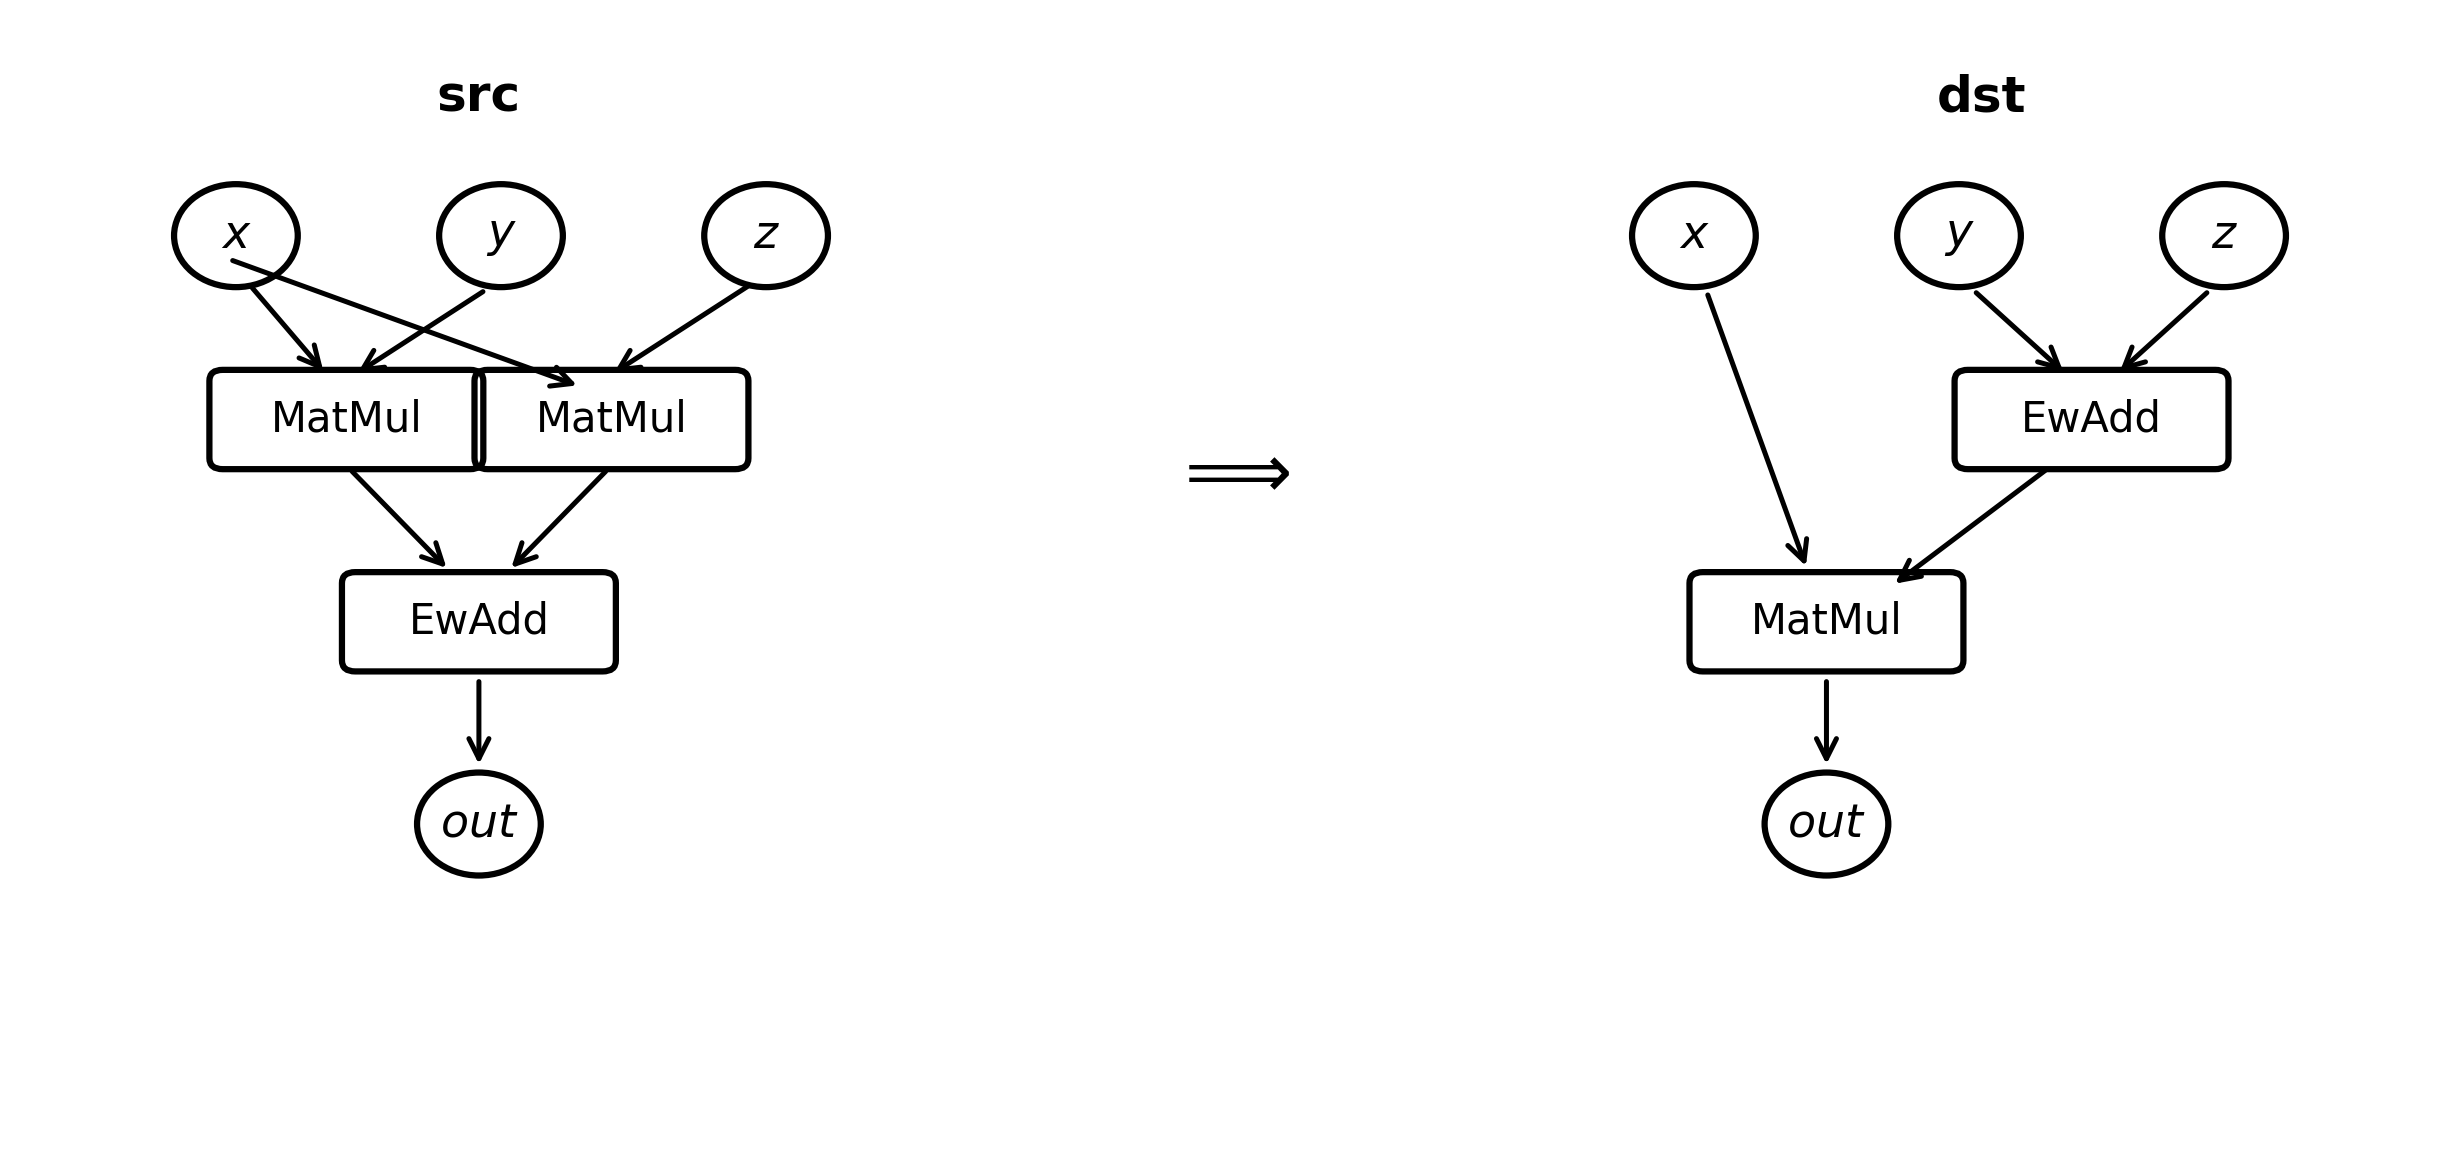
\includegraphics[width=\columnwidth]{axiom_matmul_factor_figure.png}
  \caption{Example substitution represented as a source graph and a destination graph.}
  \label{fig:axiom-matmul-factor}
\end{figure}

\subsection{Matching and Application}

Given a substitution and a target graph (the graph to which we want to apply the substitution), we first enumerate all matches of the source graph inside the target. Matching starts from a source output tensor and a candidate target tensor, and then recursively compares the two expressions, progressively building a partial match as it proceeds. Source inputs may match arbitrary target tensors, but internal source tensors must match target tensors produced by the same operator with compatible arguments. Symbolic parameters are matched in a sort-correct way, and the matching from source to target must be "decreasing" in terms of concretization (i.e. a variable in the source can match with either a variable or a literal in the target, but a literal in the source can only match with the same literal in the target). A successful match, which happens when the recursion terminates without conflict, records both a tensor map and a symbolic term map.

The tensor map is not required to be injective. This lets a source pattern such as \texttt{matmul(x,y)} match a target such as \texttt{matmul(x,x)}. This is important in practice, since several TASO substitutions rely on such surjective matches to be discovered.

Once a match has been found, we instantiate the destination side using the symbolic bindings from the match and connect its inputs to the corresponding tensors in the target graph. If the destination output is already one of those inputs, the rewrite is just a redirection. Otherwise, we insert a fresh copy of the destination fragment into the target graph and redirect the consumers of the matched source output to the new result.

A key point is that rewriting is occurrence-local. If a tensor is consumed by multiple expressions, our rewrite system must be able to rewrite only one occurrence. For example, starting from \texttt{matmul(x,x)}, the system can produce \texttt{matmul(x,transpose(transpose(x)))} by rewriting only one use of \texttt{x}. After each rewrite, we remove any now-unused bindings.

\subsection{Search}

For a target TASO substitution, our goal is to find an explicit directed derivation from one side to the other. A naive forward breadth-first search for either orientation quickly becomes infeasible, since the number of reachable graphs grows exponentially with depth.

Most of the axioms in our system are invertible, with only a small number of exceptions such as the split rules that delete tensors. We use that invertibility to speed up search. For a fixed orientation, we expand one frontier forward from the start graph and another backward from the target using inverse applications of the invertible substitutions. When the two frontiers meet, we combine the two halves into a single directed derivation. Thus, every meeting point yields a full derivation trace rather than only a reachability result.

In addition to the base axioms, our search uses a small set of derived lemmas. These are not introduced as new semantic primitives, but as proof-shortening rules that make long derivations reachable under a bounded search budget. This is consistent with TASO itself (we employ the same lemmas), which also introduces lemma-style shortcuts during verification. Interestingly, this seems to suggest that the "distance" in rewrite space and the "distance" in SMT proof space are closely related metrics.

\subsection{Canonicalization}

During search, many generated graphs differ only by tensor naming or by redundant intermediate bindings. To avoid exploring the same state repeatedly, we canonicalize every generated graph before inserting it into the search frontier. Canonicalization performs common subexpression elimination, removes bindings not reachable from the outputs, and then renames the remaining tensors deterministically. This is feasible in our setting because the graph representation has ordered inputs at each operator, so canonicalization does not need to solve a general unlabeled graph isomorphism problem.

% \section{Results}

% Overal, we are able to recover XXX/576 of all the TASO substitutions.

% TODO: add table where we show how many steps is take to get from one graph to the other, and some other empirical results.

\section{Results}
\label{sec:results}

We evaluated our system on 444 non-isomorphic substitutions extracted from the TASO implementation. A substitution was counted as recovered if our bounded search found an explicit derivation trace connecting its two sides; bidirectional frontier expansion was used only to accelerate that search. Throughout these experiments, we used a maximum search depth of 6 and a maximum number of different graphs considered of 12000.

Under this search configuration, our system recovered \textbf{432} of the \textbf{444} substitutions. This suggests that the large majority of TASO's discovered substitutions are obtainable as explicit compositions of axioms under our rewrite system. In addition, the recovered derivations were typically short. Across all 432 recovered substitutions, the mean derivation length was 2.2 steps, the median was 2, and the maximum was 6.

Table~\ref{tab:deriv-stats} summarizes the distribution of derivation lengths. Most recovered substitutions required only two rewrite steps, and only a small number required more than four. This indicates that, for most of the substitution set, the axioms do not merely imply the desired substitutions in principle, but do so through relatively short derivations.

\begin{table}[t]
\centering
\caption{Distribution of derivation lengths for recovered substitutions.}
\label{tab:deriv-stats}
\begin{tabular}{r|r}
\textbf{Steps} & \textbf{Count} \\
\hline
0 & 27 \\
1 & 67 \\
2 & 205 \\
3 & 77 \\
4 & 41 \\
5 & 13 \\
6 & 2 \\
\end{tabular}
\end{table}

The longest recovered derivations had length 6. These occurred for substitutions 155 and 308. Even these cases remained well within the search bound, while the typical substitution was recovered after only a very small number of rewrite applications.

Even this headline number should be interpreted conservatively. Recovery in our setting does not merely mean showing that two graphs are semantically equivalent or that they admit a common reduct. Rather, it requires an explicit bounded derivation trace in at least one direction. The fact that 432 of 444 substitutions satisfy this stronger criterion suggests not only that the axioms capture most of the same equalities as TASO's discovered substitution set, but also that they do so in a form that is operationally usable for directed rewriting.

% \section{Discussion, Limitations, and Next Steps}

% The major surprise was

% \subsection{Case Study}

% \paragraph{Transpose(I) $\rightarrow$ I.}
% Surprisingly, this test was initially failing due to an overly tight search budget. It turns out that this substitution, while derivable under the current axiom set, is more complicated than initially anticipated.

% \noindent\textbf{Axioms used for the derivation.}
% \begin{itemize}
% \item \texttt{axiom26: matmul(x, I) -> x}
% \item \texttt{axiom9: transpose(transpose(x)) -> x}
% \item \texttt{axiom16: transpose(matmul(x, y)) ->}\\
% \texttt{\hspace*{1.5em}matmul(transpose(y), transpose(x))}
% \end{itemize}

% \noindent In the traces below, \texttt{inv(axiom k)} means that \texttt{axiom k} is applied in the reverse direction.

% \noindent\textbf{Proof trace for \texttt{transpose(I) -> I}.}
% \begin{quote}
% \footnotesize\ttfamily
% (0) transpose(I) [start]\\
% (1) matmul(transpose(I), I) [inv(axiom26)]\\
% (2) matmul(transpose(I),\\
% \hspace*{1.8em}transpose(transpose(I))) [inv(axiom9)]\\
% (3) transpose(matmul(transpose(I),\\
% \hspace*{1.8em}I)) [inv(axiom16)]\\
% (4) transpose(transpose(I)) [axiom26]\\
% (5) I [axiom9]
% \end{quote}

% \noindent\textbf{Analogous trace for \texttt{matmul(I, x) -> x}.}
% \begin{quote}
% \footnotesize\ttfamily
% (0) matmul(I, x) [start]\\
% (1) matmul(transpose(transpose(I)),\\
% \hspace*{1.8em}x) [inv(axiom9)]\\
% (2) matmul(transpose(transpose(I)),\\
% \hspace*{1.8em}transpose(transpose(x))) [inv(axiom9)]\\
% (3) transpose(matmul(transpose(x),\\
% \hspace*{1.8em}transpose(I))) [inv(axiom16)]\\
% (4) transpose(matmul(transpose(x), I)) [lemma: transpose(I) -> I]\\
% (5) transpose(transpose(x)) [axiom26]\\
% (6) x [axiom9]
% \end{quote}

% Note that the second derivation uses \texttt{transpose(I) -> I} as a lemma, making even the shortest proof several rewrites long.

% Surprisingly, the TASO team converged on the same issue and added \texttt{Transpose(X) -> X} as a lemma when performing SMT verification for their rewrites. We adopt the same solution and enhance the axiom set with the lemmas provided by TASO.

% Interestingly, this suggests that the ``distance'' in rewrite space and the ``distance'' in SMT proof space are closely correlated.

\section{Discussion, Limitations, and Next Steps}
\label{sec:discussion}

Our results support two main conclusions. First, the large majority of TASO's discovered substitutions are obtainable by explicit composition of axioms under a powerful rewrite system. Second, these derivations are usually short. This matters because it suggests that the base axioms are not merely expressive enough in principle, but already close to the discovered substitution set in rewrite ``distance''.

At the same time, our results concern bounded recoverability rather than unrestricted derivability. The search is limited by depth and total expansion budget, and in a few places it relies on a small set of derived lemmas to shorten otherwise long proofs. The right interpretation is therefore not that we have completely characterized the closure of TASO's axiom basis, but that under a realistic explicit rewrite procedure, most of the discovered substitutions can already be reconstructed from that basis.

\subsection{Case Study: \texttt{transpose(I) \(\to\) I}}

One instructive example is the substitution \texttt{transpose(I) \(\to\) I}. Although the result is semantically simple, it is surprisingly nontrivial to recover by explicit rewriting. The derivation uses three primitive axioms:

\begin{quote}
  \small\ttfamily
  axiom26: matmul(x, I) $\rightarrow$ x\\
  axiom9: transpose(transpose(x)) $\rightarrow$ x\\
  axiom16: transpose(matmul(x, y)) $\rightarrow$\\
  \hspace*{1.5em}matmul(transpose(y), transpose(x))
  \end{quote}

Here \texttt{inv(axiom k)} denotes applying \texttt{axiom k} in the reverse direction. Under our rewrite system, one derivation is:

\begin{quote}
\small\ttfamily
(0) transpose(I) [start]\\
(1) matmul(transpose(I), I) [inv(axiom26)]\\
(2) matmul(transpose(I), transpose(transpose(I))) [inv(axiom9)]\\
(3) transpose(matmul(transpose(I), I)) [inv(axiom16)]\\
(4) transpose(transpose(I)) [axiom26]\\
(5) I [axiom9]
\end{quote}

This case illustrates an important feature of the search space induced by the axioms. Even substitutions that appear immediate at the semantic level may lie several substitution steps away when expressed only through primitive substitutions. In practice, this is one reason that a small set of derived lemmas is useful for bounded search: such lemmas do not change what is semantically derivable, but can greatly shorten the path needed to recover it.
Interestingly, this lemma was independently discovered by the TASO team when performing SMT verification for their rewrites. We thus also include their lemmas in addition to the base axioms.

% A closely related example is \texttt{matmul(I, x) \(\to\) x}, whose shortest derivation in our system naturally builds on \texttt{transpose(I) \(\to\) I} as an intermediate fact:

% \begin{quote}
% \footnotesize\ttfamily
% (0) matmul(I, x) [start]\\
% (1) matmul(transpose(transpose(I)), x) [inv(axiom9)]\\
% (2) matmul(transpose(transpose(I)), transpose(transpose(x))) [inv(axiom9)]\\
% (3) transpose(matmul(transpose(x), transpose(I))) [inv(axiom16)]\\
% (4) transpose(matmul(transpose(x), I)) [lemma: transpose(I) -> I]\\
% (5) transpose(transpose(x)) [axiom26]\\
% (6) x [axiom9]
% \end{quote}

\subsection{Case Study: A Valid but Unrecovered Rule}

One representative unrecovered substitution is the following multi-output transpose--split axis-swap rule:
\begin{quote}
\small\ttfamily
(split0\_0(transpose(concat\_1(X,Y))),\\
\hspace*{1.5em}split1\_0(transpose(concat\_1(X,Y))))\\
$\rightarrow$\\
(split0\_1(transpose(concat\_0(X,Y))),\\
\hspace*{1.5em}split1\_1(transpose(concat\_0(X,Y))))
\end{quote}
Intuitively, this rule says that transposition swaps the concatenation axis and therefore also swaps the corresponding split axis.

This substitution fails in our system for a structural reason. One way to relate the two sides is to reduce both of them to the same intermediate pair by applying the split-elimination axioms. However, those axioms are information-losing: they collapse a \texttt{split(concat(\(\cdot\),\(\cdot\)))} pattern to one branch and thereby discard the surrounding concatenation structure. Because of this, the common intermediate object can be reached only by using split elimination on both sides. That is enough for semantic equivalence, but it does not yield a clean directional rewrite from left to right or from right to left. In other words, the rule is recoverable only as a meet-in-the-middle argument, not as a single directed derivation.

This example highlights an important aspect of our task. Our goal is not merely to show that two graphs have a common reduct, but to recover a usable directional rewrite trace. For substitutions involving non-invertible, information-losing rules from both sides, these two notions can come apart. 


\subsection{Next Steps}

A natural next step is to analyze the remaining unrecovered substitutions in more detail. These failures do not all appear to have the same cause. Some, such as the multi-output split case above, reflect limitations of the current bounded search procedure and our approach to the problem. Others seem to depend on operator properties that are not yet represented in our IR or axiom basis, such as grouped-convolution semantics, or additional facts about \texttt{enlarge}, which may have been implicitly baked into the TASO verifier and approach but not mentioned in the paper. A more complete classification of these cases would sharpen the interpretation of the current recovery rate and clarify which extensions are actually necessary.

Another next step is to connect derivability back to optimization performance. If most of TASO's discovered substitutions can already be generated from the base axioms, then a natural question is whether one can optimize graphs effectively using the rewrite system itself rather than first materializing and verifying the larger substitution library, which would be a significant simplification. A direct comparison between optimization driven by explicit axiom rewriting and optimization driven by TASO's precomputed substitutions would therefore be a valuable follow-up.


\newpage
\bibliographystyle{ACM-Reference-Format}
\bibliography{refs}

\end{document}
